\documentclass[11pt,a4paper]{article}
\usepackage[margin=1in]{geometry}
\usepackage[T1]{fontenc}
\usepackage{newtxtext,newtxmath}
\usepackage{microtype,amsmath,graphicx,booktabs,tabularx}
\usepackage[numbers,sort&compress]{natbib}
\usepackage[font=small,labelfont=bf]{caption}
\usepackage{placeins}
\usepackage[hidelinks]{hyperref}
\graphicspath{{figures/}}
\hypersetup{pdftitle={Decision Models for Binary Financial Document Triage},
 pdfauthor={Lucca Pereira Martins and Matthew Ball}}
\setlength{\parskip}{0.2em}
\setlength{\emergencystretch}{2em}
\widowpenalty=10000
\clubpenalty=10000
\renewcommand{\topfraction}{0.9}
\renewcommand{\bottomfraction}{0.8}
\renewcommand{\textfraction}{0.1}
\renewcommand{\floatpagefraction}{0.75}
\title{Decision Models for Binary Financial Document Triage:\\
Adaptation, Missed Documents, and Processing Cost}
\author{Lucca Pereira Martins\thanks{Corresponding author:
 \href{mailto:lp573@cantab.ac.uk}{lp573@cantab.ac.uk}.} \and Matthew Ball}
\date{}
\begin{document}
\maketitle
\begin{abstract}
Financial document triage must trade less analyst reading against missed information and processing cost. We compare seven decision-model, finance-encoder and lexical systems under a binary source-only teacher convention. The SEC-dominated study uses 25,000 training documents, separate 1,000/500 selection/calibration cohorts and a revised 2,000-document evaluation. Trainable core systems share 4,000 documents. At 4k, Laya LoRA achieves macro F1 0.7843 versus 0.7645 for word TF-IDF/logistic. The paired F1 difference interval $[-0.0022, 0.0423]$ does not resolve an F1 difference. They miss 268 and 188 of 1543 review-worthy references, while skipping 32.4\% and 24.6\% of all documents. Laya's warm mean latency is 64.9 times the lexical classifier's on the recorded machine. Larger training subsets separately measure sample efficiency, and calibration-selected skip policies expose workload/miss tradeoffs. The test reuses previously inspected documents; these results measure teacher agreement, not independent confirmation or analyst-validated materiality. We provide inspectable labels, predictions and independent CPU replay.

\end{abstract}

\section{Introduction}
Financial document triage assigns incoming information to automatic discard or
analyst review. The useful outcome is less reading with few missed developments,
at a processing cost compatible with the incoming volume. A model that sends
everything to review avoids false negatives but removes no work. Conversely,
fast classification is unhelpful if it discards information the analyst should see.

We study a binary, source-content-only review convention across public financial
filings, corporate releases, policy announcements and a smaller news sample.
The two labels are \emph{routine} and \emph{review-worthy}. An unresolved,
potentially significant financial development goes to review; uncertainty is
metadata rather than a third routing destination. Historical company context,
portfolio exposures and subsequent returns are unavailable to the classifier.
The reference labels therefore define a review convention, rather than establish
investment materiality.

Our main question is whether adaptation of a pretrained decision model improves
this task relative to a finance encoder and a lexical classifier, and whether
any improvement warrants its measured processing cost. Seven systems form the
core comparison: native Laya, Laya with head adaptation, Laya with low-rank
adaptation (LoRA), frozen FinBERT with logistic regression, FinBERT with LoRA,
word TF-IDF with logistic regression, and a training-majority reference.
Trained core systems share the same 4,000 documents. Larger training subsets
address sample efficiency separately from this equal-data comparison.

The contribution is an incremental financial-domain benchmark with explicit
reference provenance, event-group controls, adaptation controls and inspectable
workload/resource measurements. The study follows an earlier three-class
exploration and reuses its test documents. All binary model and policy choices
are frozen before the revised evaluation, but this is not a fresh independent
confirmation of the earlier findings. We report that boundary alongside the
teacher-agreement nature of the task.

\section{Related work}
Financial relevance filtering is established. Ahbali et al.\ \citep{credit}
use a TF-IDF/SVM relevance filter before corporate credit-event analysis.
Del Corro and Hoffart \citep{financialrelevance} derive financial-news relevance
from stock-prediction attention. FinLin \citep{finlin} provides multi-source,
expert-annotated entity relevance and sentiment. These targets differ from
whole-document source-only review triage.

Closely related decision-model studies also exist. Nandakishore
\citep{assessor} evaluates Laya Typed-Decisions, teacher agreement, calibration
and selective escalation on synthetic workflows. Stuani's engineering
benchmark \citep{complaints} compares Laya, lexical classifiers, encoders and
language models on financial complaint routing and fraud flags. Borchers
\citep{borchers} compares adapted decision models with frozen representations
and learning curves on research-paper categories. Our task and corpus differ;
we do not claim to introduce financial filtering, decision-model comparison
or calibration analysis.

Laya's English root checkpoint uses ModernBERT-large and a learned typed-decision
head \citep{laya,modernbert}. FinBERT's adaptation to financial text and sentiment
\citep{finbert} makes it a relevant industry comparator, but its sentiment head
does not supply review labels. We use its encoder with a task classifier.
LoRA \citep{lora} and temperature scaling \citep{guo} are established methods.
Automated annotation still requires task-specific validation \citep{annotation};
success on another annotation task does not validate this rubric.

\section{Task and data}
\label{sec:data}
The classifier receives the extracted English source body. Clearly ordinary or
administrative content is routine. A potentially significant financial development,
including an unresolved one, warrants review. A scheduled release can carry important
information; positive or negative sentiment alone does not determine review.
Neither issuer-specific history nor source identifiers are additional model features.
Source and event metadata support acquisition, grouping and evaluation.

The corpus draws from SEC filings and release exhibits, Federal Reserve releases,
ECB institutional/statistical releases, GOV.UK announcements and Wikinews.
It contains 25,000 training documents dated through March 2026, 1,000 selection
and 500 calibration documents from April--June, and 2,000 test documents from
July--September. Related-document groups do not cross these cohorts. Source
coverage follows eligible available documents; there is no ECB quota.
The added ECB collection supplies 534 English institutional/statistical releases,
with author-named and third-party content excluded. Publication/body snapshots
are retained with hashes and attribution.
For 350 retained training filings, edgartools supplied the captured text;
their public links identify verified parent SEC submissions.

Existing definite references are retained. Luna Flex freshly decides every
previously unclear reference and labels newly selected documents using a pinned
binary rubric. Thus \emph{unclear} is not mapped mechanically into either class.
A blinded, balanced 200-document training-only consistency audit compares the
retained references with binary decisions; it does not override them. This is a
hybrid annotation protocol, and the audit measures teacher consistency rather
than agreement with financial analysts. Teacher-reported uncertainty is neither
a ground-truth error probability nor an evaluation class.

Evaluation additions are chosen without labels or model scores, retaining the
earlier selection/calibration/test memberships. The revised test keeps the
previous 1,800 bodies and adds 200. Group checks exclude exact matches,
known event aliases and verified near-duplicates; probabilistic candidate
retrieval and inherited groups can miss relationships. Unselected raw corpora
are not exhaustively re-clustered. SEC content remains dominant, and the small
news component does not represent a general news inbox.

\begin{table}[!htbp]
\centering
\caption{Frozen cohort support. The test retains 1,800 earlier bodies; reference labels are revised.}
\label{tab:data}
\small
\setlength{\tabcolsep}{3.5pt}
\begin{tabularx}{\linewidth}{@{}Xrrrrrr@{}}
\toprule
Cohort & Documents & Routine & Review & Groups & SEC & ECB\\
\midrule
Train & 25000 & 7173 & 17827 & 24696 & 20740 & 1175\\
Selection & 1000 & 283 & 717 & 993 & 889 & 29\\
Calibration & 500 & 135 & 365 & 493 & 461 & 12\\
Test & 2000 & 457 & 1543 & 1967 & 1870 & 40\\
\bottomrule
\end{tabularx}
\end{table}


\section{Systems and evaluation}
\label{sec:methods}
\subsection{Fixed comparisons and adaptation}
Training subsets of 4,000, 16,000 and 25,000 documents are nested, with stable
round-robin family/class sampling. All trainable core systems use the same
4,000 bodies; the majority reference counts the same labels without optimization. Native Laya
requires no task training. TF-IDF and frozen FinBERT/logistic additionally use
16,000 and 25,000 training documents. FinBERT LoRA uses 16,000; Laya LoRA at
that size is admitted only when its measured runtime fits the compute deadline.
No 25,000-document LoRA run enters this study. Every learning-curve point also
uses the same 1,500 development labels; training count is not total annotation cost.

TF-IDF learns its vocabulary and transforms from training alone. Logistic
regularization and class weighting use the same bounded grid at each training
size, selected by selection macro F1 (Appendix~\ref{sec:supporting}).
Frozen FinBERT features are computed once and cached with
body, recipe and source identities; encoding cost is reported separately from
classifier fitting and cache reuse. Frozen encoder windows are averaged and
L2-normalized before classification.

We use pinned \texttt{convaiinnovations/laya} English root and
\texttt{ProsusAI/finbert} checkpoints; full revisions accompany the evidence.
Adapted neural systems use seed 42, unweighted document-level cross-entropy and
up to three epochs. Raw selection macro F1 chooses the checkpoint; epoch zero
is eligible, and ties retain the earlier epoch. Laya head adaptation updates
the decision head with a frozen encoder at learning rate $3\times10^{-5}$.
LoRA updates rank-eight encoder adapters and the task head at $10^{-4}$, with
scaling 16 and adapter dropout 0.05. Matched pre-update states are preserved
as supporting controls, avoiding a direct attribution of every SDK-to-adapted
change to weight updates.

Laya adaptation uses a 1,024-token context and FinBERT uses 512. Overlapping
windows cover all normalized source tokens, and uniform window-logit pooling
gives one document-level prediction and loss. No window labels are inferred.
The native Laya SDK limits GPU passes to eight windows, retaining its own
long-document aggregation, so it differs from
adapted Laya in pooling as well as fitting. Architectures, parameter counts,
pretraining objectives and classifier recipes differ across systems; those
comparisons cannot isolate finance pretraining or LoRA as a sole cause.

\subsection{Agreement, misses and review workload}
Macro F1 averages the routine and review-worthy class F1 values. Exact binary
ties route to review. We also report review precision/recall, the $2\times2$
confusion matrix, and false negatives divided by review-worthy reference
support. At the default decision, a document predicted routine is skipped.
The skipped fraction quantifies reading removed; its complement is review
workload. A low miss rate can reflect more review rather than better
discrimination, so both quantities accompany every operational comparison.

Scalar temperature is fit by calibration negative log likelihood. It changes
confidence while preserving the default class decision. Binary Brier score is
the sum over both class columns, equal to twice the positive-class squared
error. We report raw/calibrated scoring arithmetic in the evidence package.

We fit five routine-only skip policies on calibration: empirical review-miss
targets of 1\% and 5\%, and maximum skip budgets of 10\%, 20\% and 30\%.
Each chooses the largest feasible calibration skip count without splitting
equal-probability ties. Predicted review documents are never skipped by these
rules. We report achieved test skip counts and missed references, rather than
assume workloads match or that fitting targets are population guarantees.

The fixed primary comparison is 4k Laya LoRA versus 4k word TF-IDF/logistic.
We use 2,000 paired whole-group bootstrap draws for percentile 95\% intervals
and their differences. These intervals condition on a single fitted run;
they do not measure training instability or correct supplementary comparisons
for multiplicity. Source/length slices are descriptive, with support reported.
No method, checkpoint or policy is selected using revised-cohort outcomes.

\subsection{Measured resources}
GPU jobs run serially on an NVIDIA RTX 3060 with 12 GiB GPU memory;
CPU work uses an Intel Core i5-12400F. Warm inference includes tokenization/windowing and
classification, excludes model loading, and uses the same 128 selection bodies.
We retain each latency, mean/P95, batch-throughput denominator and peak allocated
GPU memory. Neural fitting time and successful command elapsed time are distinguished;
interrupted attempts are accounted for separately.
Frozen feature preparation/cache measurements accompany classifier fitting.
Local timings on the recorded hardware do not estimate cloud prices, energy
use or deployment service latency.

\FloatBarrier
\section{Results}
\label{sec:results}
\subsection{Equal-data system comparison}

Laya LoRA has the highest 4k macro F1 point estimate in Table~\ref{tab:main}. The prespecified Laya-minus-TF-IDF contrast is 0.0199 with paired 95\% interval $[-0.0022, 0.0423]$. The interval includes zero and does not establish equivalence. At default decisions, Laya skips 156 additional documents but misses 80 more review-worthy references. Its review precision is 94.3\% versus 89.9\%, while recall is 82.6\% versus 87.8\%. The higher macro F1 therefore does not imply fewer missed developments. Laya's warm mean inference latency is 64.9 times the lexical classifier's.

\begin{table}[!htbp]
\centering
\caption{Core systems on the revised 2,000-document evaluation. Default decisions; false negatives (FN) are divided by review-reference support. All trainable systems use the same 4k bodies; majority counts those labels, and SDK has no task fit. Warm inference includes full document processing.}
\label{tab:main}
\small
\setlength{\tabcolsep}{3.5pt}
\begin{tabularx}{\linewidth}{@{}Xrrrrr@{}}
\toprule
System & F1 (95\% CI) & FN & Skipped & Mean ms & P95 ms\\
\midrule
Training majority & 0.436 $[0.429, 0.441]$ & 0/1543 & 0.0\% & 2.97 & 3.45\\
Word TF-IDF/logistic & 0.764 $[0.743, 0.786]$ & 188/1543 & 24.6\% & 4.58 & 8.16\\
Frozen FinBERT/logistic & 0.718 $[0.696, 0.740]$ & 302/1543 & 30.9\% & 35.81 & 113.33\\
FinBERT LoRA & 0.743 $[0.721, 0.763]$ & 352/1543 & 36.5\% & 35.17 & 116.72\\
Laya native SDK & 0.542 $[0.519, 0.567]$ & 96/1543 & 8.3\% & 334.22 & 1332.02\\
Laya head & 0.609 $[0.587, 0.632]$ & 473/1543 & 37.3\% & 276.66 & 1131.21\\
Laya LoRA & 0.784 $[0.764, 0.805]$ & 268/1543 & 32.4\% & 297.19 & 1207.55\\
\bottomrule
\end{tabularx}
\end{table}

\begin{figure}[tbp]\centering
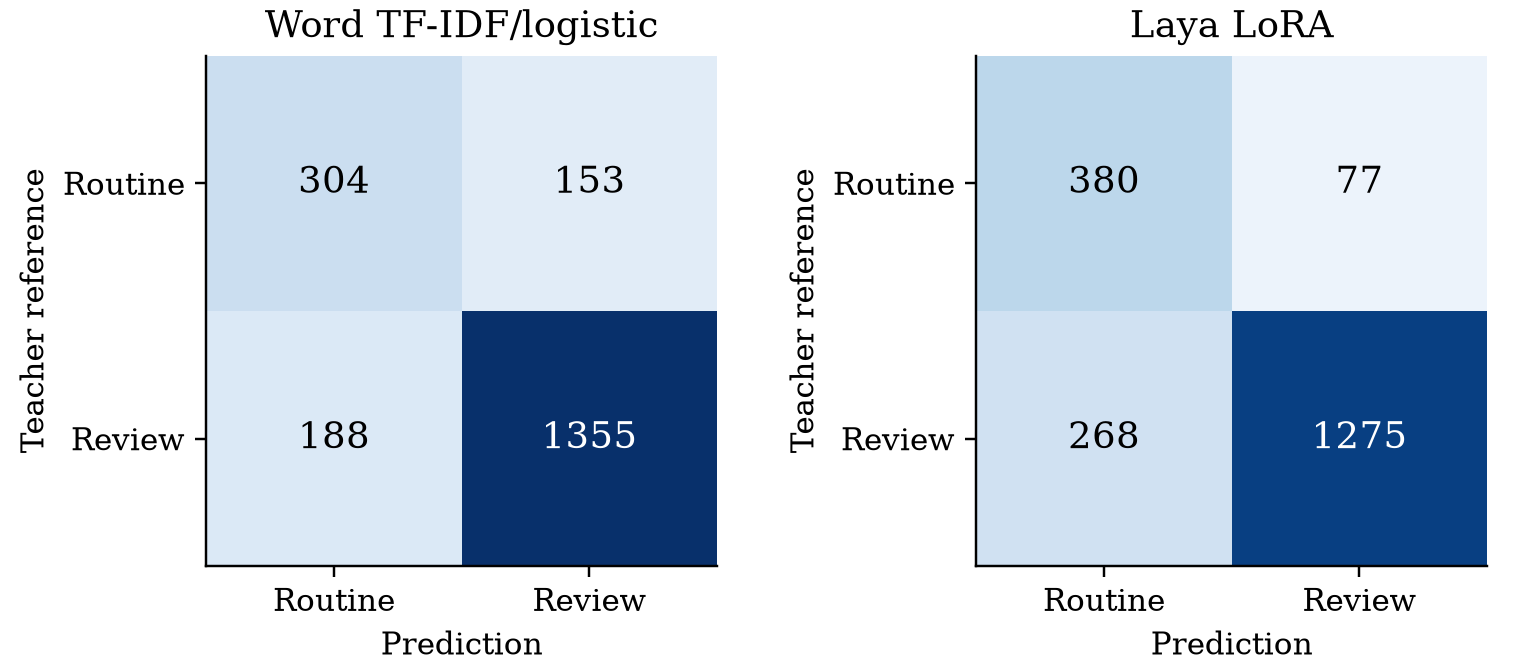
\includegraphics[width=\linewidth]{confusion.png}
\caption{Default two-class confusion matrices for the fixed primary pair. Rows are teacher references; columns are model predictions. Counts sum to 2,000 in each matrix.}\label{fig:confusion}\end{figure}

\subsection{Review workload and missed references}

Table~\ref{tab:policy} applies calibration-selected thresholds unchanged to test. The 1\% fitting target and 20\% skip budget produce different achieved workloads across systems; neither is a test guarantee. For the primary pair, the 1\% calibration miss target reduces skipped test reading to 2.5\% for Laya and 6.2\% for TF-IDF. Stringent miss control removes much of the workload reduction apparent at default decisions. A lower achieved miss count cannot be interpreted independently of how much reading remains.

\begin{table}[!htbp]
\centering
\caption{Achieved test outcomes for two calibration policies. The left pair uses an empirical 1\% calibration miss target; the right pair maximizes calibration skips within 20\%. All policies skip only routine predictions and preserve ties. Achieved test workloads are not assumed equal.}
\label{tab:policy}
\small
\setlength{\tabcolsep}{3.5pt}
\begin{tabularx}{\linewidth}{@{}Xrrrr@{}}
\toprule
System & 1\% miss: FN & Skipped & 20\% skip: FN & Skipped\\
\midrule
Training majority & 0/1543 & 0.0\% & 0/1543 & 0.0\%\\
Word TF-IDF/logistic & 20/1543 & 6.2\% & 95/1543 & 15.8\%\\
Frozen FinBERT/logistic & 27/1543 & 4.0\% & 159/1543 & 18.7\%\\
FinBERT LoRA & 31/1543 & 5.3\% & 144/1543 & 19.8\%\\
Laya native SDK & 14/1543 & 0.9\% & 95/1543 & 8.2\%\\
Laya head & 14/1543 & 1.4\% & 240/1543 & 19.6\%\\
Laya LoRA & 7/1543 & 2.5\% & 124/1543 & 19.7\%\\
\bottomrule
\end{tabularx}
\end{table}

\subsection{Adaptation and sample efficiency}

Figure~\ref{fig:learning} separates training size from the shared-4k comparison. Intervals are conditional on fixed fitted runs and are not corrected for multiple comparisons. Training source/class composition and optimization steps also change across sizes; these are fixed-recipe curves, rather than a causal estimate of sample count alone.

\begin{figure}[tbp]\centering
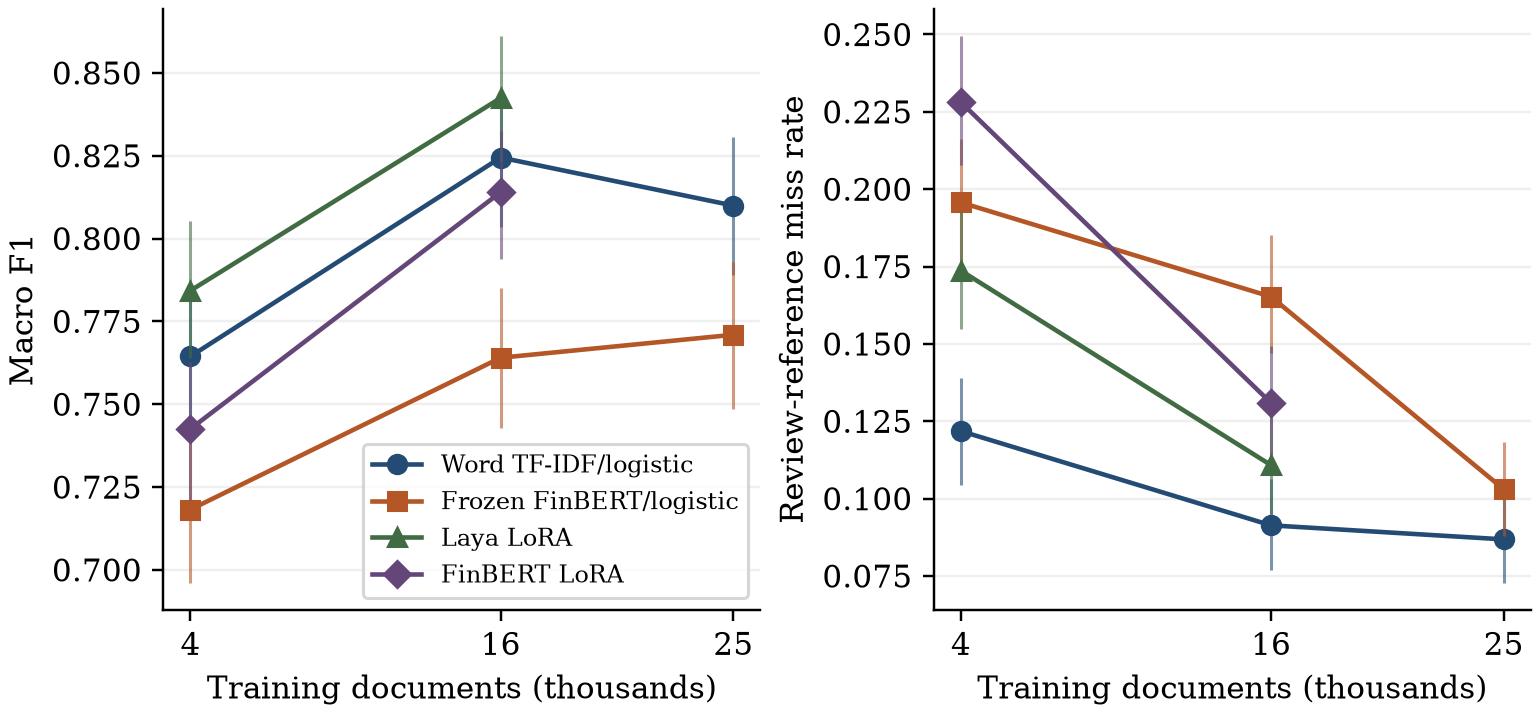
\includegraphics[width=\linewidth]{learning-curves.png}
\caption{Nested training-size curves for completed recipes. Left: macro F1. Right: review-reference miss rate at default decisions. Vertical segments are marginal whole-group 95\% intervals. LoRA curves stop at 16,000 training documents.}\label{fig:learning}\end{figure}

At 16k, Laya LoRA reaches F1 0.8424 and word TF-IDF/logistic 0.8245; FinBERT LoRA reaches 0.8140. Laya and TF-IDF default miss counts are 171 and 141, with 28.0\% and 24.3\% skipped. The successful commands take 20.66 hours and 59.5 seconds, respectively; FinBERT LoRA takes 2.51 hours. These larger-run point estimates supplement the fixed 4k primary comparison; they do not replace it.

The matched pre-update comparisons in Table~\ref{tab:controls} separate task fitting from context, pooling and initial-head differences. Each recipe is compared with its own preserved initial state. These controls do not isolate pretraining or equalize classifier budgets across model families.

The primary systems share 122 default missed references, with 146 additional Laya-only and 66 TF-IDF-only misses. This overlap describes the fixed predictions; it does not evaluate a new combined routing rule.

\begin{table}[!htbp]
\centering
\caption{Paired training-size F1 increments for fixed system families. Conditional 95\% intervals; supplementary comparisons are uncorrected.}
\label{tab:increments}
\small
\setlength{\tabcolsep}{3.5pt}
\begin{tabularx}{\linewidth}{@{}XXrr@{}}
\toprule
System & Training change & $\Delta$ F1 & 95\% interval\\
\midrule
Word TF-IDF/logistic & 4k to 16k & 0.0600 & $[0.0421, 0.0795]$\\
Word TF-IDF/logistic & 16k to 25k & -0.0145 & $[-0.0295, 0.0013]$\\
Frozen FinBERT/logistic & 4k to 16k & 0.0458 & $[0.0292, 0.0624]$\\
Frozen FinBERT/logistic & 16k to 25k & 0.0069 & $[-0.0098, 0.0230]$\\
Laya LoRA & 4k to 16k & 0.0581 & $[0.0428, 0.0735]$\\
FinBERT LoRA & 4k to 16k & 0.0715 & $[0.0535, 0.0899]$\\
\bottomrule
\end{tabularx}
\end{table}


\section{Discussion and limitations}
The lexical classifier remains a credible low-cost reference on this benchmark. Laya adaptation improves agreement relative to its matched initial state, but greater reading reduction at default decisions also brings additional misses. A triage operating point therefore needs an explicit miss/workload objective fixed before evaluation; a macro F1 ranking alone cannot determine it. The training-only reference audit agrees on 93.0\% of 200 balanced retained labels. That consistency result cannot substitute for expert reference validity or estimate a population annotation error rate.

The reference convention is the central limit. Training and evaluation share
a teacher, and retained versus newly decided labels use different protocols.
Independent expert adjudication is needed before treating a teacher miss as
an economically material miss. Review priorities also depend on company,
portfolio and historical context absent from these inputs. No trading strategy
or investment profitability is evaluated.

The revised evaluation is temporally later but reuses previously inspected
test bodies. Fixing binary choices before the rerun prevents selection on its
new scores; it does not erase earlier information or create independent
confirmation. Fresh representative evaluation data would be needed for that
claim. Source imbalance, public-document selection, revised historical web
content, possible pretraining exposure and missed duplicate relationships
further constrain transfer to industry inboxes.

The fixed recipes answer a bounded comparison, not the best achievable score
for every model family. One fitted seed leaves optimization variability
unmeasured. Supplementary scaling/control intervals are uncorrected, and
calibration operating points can shift with source mix. The study includes
neither a frontier generative classifier nor full-model adaptation or RLCD
training. It should guide a narrower next experiment, rather than establish
a universal model ranking.

\section{Conclusion}
On this SEC-dominated teacher benchmark, LoRA improves Laya relative to matched pre-update states and benefits from the larger training subset. The prespecified 4k comparison does not establish an F1 advantage over word TF-IDF/logistic; Laya's additional default skipping comes with more missed references and substantially higher measured processing cost. Calibration exposes how stringent miss control reduces reading removed. Expert reference validation and a fresh representative evaluation cohort are needed before operational generalization claims.


\section*{Code and reproducibility}
The public repository supplies a separate binary evidence package with ordered
references/logits, decisions, fitting histories, resource measurements,
artifact/source identities and independent CPU arithmetic replay. Exact model
fitting additionally requires the preserved local bodies, checkpoints and
pinned pretrained weights. Public source URLs identify the documents, but live
recollection does not guarantee identical historical text. Attribution and transfer conditions accompany collection
code; bodies and weights are excluded from the public evidence package.
The earlier three-class study and its scientific bundles remain preserved.
The command \texttt{python decision\_models/reports/binary-v2/verify.py} replays the published metrics, policies, timing summaries and paired intervals on CPU without API calls. Code and evidence are available in the \href{https://github.com/LuccaPereiraMartins/systematic-trading/tree/codex/research-binary-paper/decision_models/reports/binary-v2}{versioned study package}. The revised freeze identity is \texttt{e6afdaf08581}; its full hash and source identities accompany the package.


\FloatBarrier
\begin{thebibliography}{99}
\small
\bibitem{finbert}
Dogu Araci.
FinBERT: Financial sentiment analysis with pre-trained language models.
2019. \href{https://arxiv.org/abs/1908.10063}{arXiv:1908.10063}.

\bibitem{modernbert}
Benjamin Warner et al.
Smarter, better, faster, longer: A modern bidirectional encoder for fast,
memory efficient, and long context finetuning and inference.
2024. \href{https://arxiv.org/abs/2412.13663}{arXiv:2412.13663}.

\bibitem{laya}
ConvAI Innovations.
\emph{Laya model card}, pinned English root checkpoint.
\url{https://huggingface.co/convaiinnovations/laya}.
Checkpoint revision \texttt{55cf4c4ebb4e}; accessed October 2026.

\bibitem{lora}
Edward J. Hu, Yelong Shen, Phillip Wallis, Zeyuan Allen-Zhu, Yuanzhi Li,
Shean Wang, Lu Wang, and Weizhu Chen.
LoRA: Low-rank adaptation of large language models.
2021. \href{https://arxiv.org/abs/2106.09685}{arXiv:2106.09685}.

\bibitem{guo}
Chuan Guo, Geoff Pleiss, Yu Sun, and Kilian Q. Weinberger.
On calibration of modern neural networks.
In \emph{Proceedings of the 34th International Conference on Machine Learning},
2017. \href{https://arxiv.org/abs/1706.04599}{arXiv:1706.04599}.

\bibitem{annotation}
Nicholas Pangakis, Samuel Wolken, and Neil Fasching.
Automated annotation with generative AI requires validation.
2023. \href{https://arxiv.org/abs/2306.00176}{arXiv:2306.00176}.

\bibitem{credit}
Noujoud Ahbali, Xinyuan Liu, Albert Aristotle Nanda, Jamie Stark, Ashit Talukder,
and Rupinder Paul Khandpur.
Identifying corporate credit risk sentiments from financial news.
In \emph{Proceedings of NAACL-HLT 2022: Industry Track Papers},
pp.\ 362--370, 2022. \url{https://aclanthology.org/2022.naacl-industry.40/}.

\bibitem{financialrelevance}
Luciano Del Corro and Johannes Hoffart.
From stock prediction to financial relevance: Repurposing attention weights
to assess news relevance without manual annotations.
2020. \href{https://arxiv.org/abs/2001.09466}{arXiv:2001.09466}.

\bibitem{finlin}
Tobias Daudert.
A multi-source entity-level sentiment corpus for the financial domain:
the FinLin corpus.
\emph{Language Resources and Evaluation}, 56:333--356, 2022
(first published online 2021).
\href{https://doi.org/10.1007/s10579-021-09555-3}{doi:10.1007/s10579-021-09555-3}.

\bibitem{assessor}
Gowthamkumar Nandakishore.
Laya as a typed probabilistic assessor: An independent reproduction and a
preregistered study of calibration and selective escalation.
2026. \href{https://arxiv.org/abs/2609.33843}{arXiv:2609.33843}.

\bibitem{complaints}
Eduardo Stuani.
Laya vs LLMs: Picking the right model for financial complaint triage.
Public engineering benchmark, 2026.
\url{https://github.com/stuaninauts/bench-laya-vs-llms}.
Repository snapshot \texttt{95cdee3e8539}; accessed 13 October 2026.

\bibitem{borchers}
Oliver Borchers.
Do you even need a decision model?
Engineering benchmark report, 4 October 2026; updated 7 October.
\url{https://www.drborchers.com/en/blog/do-you-need-a-decision-model/}.
\end{thebibliography}

\clearpage
\appendix
\section{Supporting comparisons and provenance}
\label{sec:supporting}
The following tables support the main agreement/workload questions: recipes,
pre-update controls and fitting resources. Full calibration policies,
descriptive source/length/reference-basis slices and per-document arithmetic
are retained in the public evidence package with their audit receipts.
The linear grid uses $C\in\{0.001,\allowbreak0.01,\allowbreak0.1,\allowbreak1,\allowbreak10,\allowbreak30,\allowbreak100\}$
and either no class weighting or balanced weights.
\begin{table}[!htbp]
\centering
\caption{Matched pre-update comparisons. The initial adapted pooling/head state is the control; it is distinct from native SDK inference. Larger fixed recipes reuse a matched setup's pre-update control. Intervals are supplementary.}
\label{tab:controls}
\small
\setlength{\tabcolsep}{3.5pt}
\begin{tabularx}{\linewidth}{@{}Xrrrr@{}}
\toprule
System & Train & Zero F1 & Fit F1 & $\Delta$ F1 interval\\
\midrule
Laya head & 4k & 0.557 & 0.609 & $[0.023, 0.083]$\\
Laya LoRA & 4k & 0.557 & 0.784 & $[0.196, 0.259]$\\
FinBERT LoRA & 4k & 0.187 & 0.743 & $[0.535, 0.574]$\\
FinBERT LoRA & 16k & 0.187 & 0.814 & $[0.607, 0.646]$\\
Laya LoRA & 16k & 0.557 & 0.842 & $[0.255, 0.316]$\\
\bottomrule
\end{tabularx}
\end{table}

\begin{table}[!htbp]
\centering
\caption{Completed neural configurations. All use seed 42 and at most three epochs; epoch zero is eligible. A context limit includes task/model overhead, rather than denote full source coverage. All normalized source tokens are windowed.}
\label{tab:recipes}
\small
\setlength{\tabcolsep}{3.5pt}
\begin{tabularx}{\linewidth}{@{}Xrrrr@{}}
\toprule
System & Train & Context & Trainable & Selected epoch\\
\midrule
Laya head & 4k & 1024 & 26248193 & 2\\
Laya LoRA & 4k & 1024 & 27165697 & 3\\
FinBERT LoRA & 4k & 512 & 297986 & 3\\
FinBERT LoRA & 16k & 512 & 297986 & 3\\
Laya LoRA & 16k & 1024 & 27165697 & 3\\
\bottomrule
\end{tabularx}
\end{table}

\begin{table}[!htbp]
\centering
\caption{Recorded resources. Command time includes preparation, fitting and development evaluation. Fit phase is the neural history or linear preparation/search duration, including selection overhead. Fit GiB records neural-fit peaks only; '--' denotes an unavailable measurement. Inference peaks can include resident fitting state. Frozen feature/cache costs are included in command time and itemized in the evidence.}
\label{tab:resources}
\small
\setlength{\tabcolsep}{3.5pt}
\begin{tabularx}{\linewidth}{@{}Xrrrrr@{}}
\toprule
System & Train & Command s & Fit phase s & Fit GiB & Infer GiB\\
\midrule
Training majority & Count 4k & 6.3 & 0.2 & -- & 0.00\\
Word TF-IDF/logistic & 4k & 22.9 & 15.9 & -- & 0.00\\
Frozen FinBERT/logistic & 4k & 219.1 & 199.1 & -- & 0.51\\
Laya native SDK & None & 812.9 & -- & -- & 2.35\\
Laya head & 4k & 9225.8 & 8541.7 & 2.37 & 2.10\\
Laya LoRA & 4k & 17014.8 & 16278.2 & 3.24 & 2.12\\
FinBERT LoRA & 4k & 2209.4 & 2099.5 & 0.78 & 0.52\\
Word TF-IDF/logistic & 16k & 59.5 & 51.8 & -- & 0.00\\
Word TF-IDF/logistic & 25k & 97.2 & 89.8 & -- & 0.00\\
Frozen FinBERT/logistic & 16k & 485.9 & 465.4 & -- & 0.51\\
Frozen FinBERT/logistic & 25k & 481.5 & 459.2 & -- & 0.51\\
FinBERT LoRA & 16k & 9043.6 & 8951.9 & 0.79 & 0.52\\
Laya LoRA & 16k & 74374.3 & 73637.6 & 3.24 & 2.12\\
\bottomrule
\end{tabularx}
\end{table}

\FloatBarrier
Laya native SDK also used 886.0 seconds in prior interrupted attempts. These attempts are excluded from the successful-command column; cumulative elapsed time and attempt receipts remain in the evidence package.

\end{document}
